\chapter{Making Sense of Reasoning Relationships through User Actions}
\label{chap:sensepath}

\graphicspath{{Chapter5/figures/}}

\begin{figure}[!h]
	\centering
	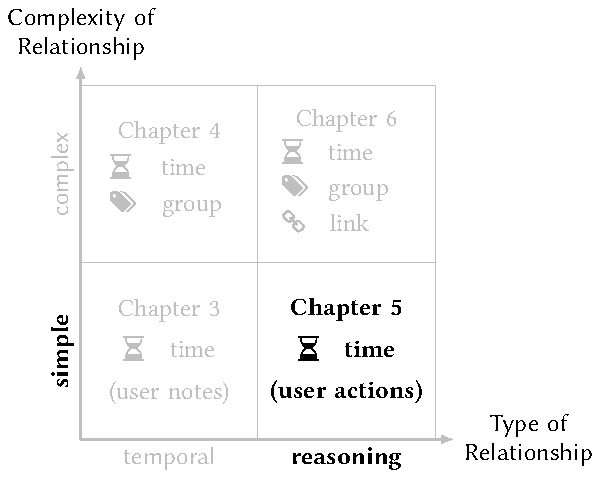
\includegraphics{work}
\end{figure}

\vspace{.8in}

\blfootnote{Published in \emph{IEEE Transactions on Visualization and Computer Graphics}~\cite{Nguyen2016}.}
\blfootnote{Demo video is available at: \url{https://vimeo.com/144641566}.}

\pagebreak

\lettrine{C}{hapter} \ref{chap:schemaline} and \autoref{chap:timesets} discussed how to support users to explore temporal relationships of sensemaking through interactive timeline visualizations of their annotations. However, the relationship that emerges in the sensemaking process could be more complicated than a temporal one. Besides understanding how events are connected, getting to know why they happened in such order is also important. This chapter investigates how to support users to explore such a reasoning relationships of sensemaking though visualization of provenance data. Qualitative research methods are often used to gain understanding about this kind of relationship. Such a research process is highly manual and time-consuming: researchers collect observation data, transcribe screen capture videos and think-aloud recordings, identify recurring patterns, and eventually abstract the sensemaking process into a general model. This chapter contributes a visualization tool -- \emph{SensePath} -- that facilitates the exploration of reasoning relationships in sensemaking, focusing on qualitative research.

The previous two chapters visualize annotations made by users. Even though these annotations often contain high-level thinking by users, these information resources are limited. This is because making detailed and frequent notes requires a huge amount of time and effort from the users. Also, it may distract them from their sensemaking tasks. This chapter focuses on exploring \emph{reasoning relationship} of sensemaking through both \emph{user annotations} and automatically captured \emph{user actions}. SensePath provides multi-linked visualizations of the captured provenance and interactive features to support analysis. Two user-centered evaluations were conducted to explore how the tool would be used and identify any benefits it could provide. The participants were able to gain deep understanding of the sensemaking processes in relatively short time.

\section{Introduction}
Sensemaking is described as the process of comprehension, finding meaning and gaining insight from information, producing new knowledge and informing action~\cite{Pirolli2005}. Given the rapid increase in data volume and complexity, more tools are needed to support sensemaking, which in many cases remains a slow and laborious process performed by human analysts. The design of such tools requires a deep understanding of the sensemaking process, which is a reoccurring goal of qualitative research conducted by many HCI researchers. Common methods for such qualitative analyses are grounded theory~\cite{Corbin1994} and thematic analysis~\cite{Guest2011}. Typically, researchers need to design a study, collect observation data, transcribe the screen capture videos and think-aloud recordings, identify interesting patterns, group them into categories, and build a model or theory to explain those findings. Unfortunately, this process largely remains manual and thus very time consuming.

In this chapter, we introduce a visual analysis tool SensePath to help HCI researchers recover user's thinking using analytic provenance information. More specifically, we support thematic analysis of online browser-based sensemaking tasks. We chose this domain because many of the everyday sensemaking tasks such as travel planning, are now performed online~\cite{Russell2008}. The design of SensePath is based on the observation of a number of sensemaking sessions and the post hoc analyses that researchers performed to recover the sensemaking process. This is followed by a participatory design session with HCI researchers that led to a number of design requirements such as supporting reasonably long sensemaking tasks (up to two hours), integration with existing qualitative analysis workflow, and non-intrusiveness for participants. 

As a result, SensePath was designed to target the \emph{transcription} and \emph{coding} phases during which a researcher needs to transcribe the observation data, such as screen capture video and think-aloud recording (transcription), and then identify the common themes of the sensemaking actions within them and assign appropriate names (coding). SensePath consists of two components designed for different stages of thematic analysis: one runs in the background during the observation to automatically capture analytic provenance, which includes sensemaking actions; the other component is designed for post hoc analysis phase and it visualizes the recorded information in four linked views to help transcription, coding, and identify frequent patterns and high level sense-making process. While some features are tailored for sensemaking, the general approach of understanding user's thinking can be applied to a wider qualitative research. Also, SensePath can be extended to support the analysis of other online activities, not limited to sensemaking tasks. 

Two evaluations were conducted to understand how the tool was used by experienced HCI researchers and to discover whether and how SensePath provides any advantages to the analyst compared to traditional analysis methods. The researchers found the tool intuitive and considerably reduces the analysis time, enabling the discovery of underlying sensemaking processes. 

In summary, this chapter contributes
\begin{itemize}
\item A qualitative study and a participatory design session to understand characteristics of qualitative research on sensemaking.
\item A visual analysis tool SensePath enabling researchers to explore rational relationship of a user's sensemaking process. It supports the transcription and coding of the observation data of online sensemaking tasks and can be potentially applied to other qualitative research in HCI beyond sensemaking. 
\item A qualitative user evaluation that demonstrated the effectiveness of the general approach and the tool SensePath.
\end{itemize}
\section{Related Work on Qualitative Research}
Qualitative research methodologies~\cite{Adams2008} are typically used in study of sensemaking. They allow researchers to reveal often complex user experiences and understand issues that are experienced subjectively or collectively~\cite{Pace2004, Adams2008}. Moreover, sensemaking research is often concerned not with testing an existing theory, but building a new one through the collection and analysis of relevant data, generating new knowledge about users and the usage of technology~\cite{Rogers2012}.

Inductive approaches to qualitative research are commonly applied, such as grounded theory~\cite{Corbin1994}, content analysis~\cite{Stemler2001}, and thematic analysis~\cite{Guest2011}. They rely on the interpretation of rich textual and multimedia data, through manual processing of data and coding before describing it in the context of categories or themes. Furthermore, in the case of multimedia data, transcription of audio or video data is often also required. Though these approaches lead to important insights, they are labor intensive, time-consuming and costly in their application~\cite{Wong2002}. Software packages are designed to provide qualitative researchers useful ways to code and index data, and manage the evolving complexity of the process~\cite{Lewins2007}. However, a qualitative analysis is still a largely manual process requiring a substantial investment of time and resources in leading to insightful findings.



\section{Approach}
This section discusses our approach to understand and elicit user requirements.

\subsection{Qualitative Analysis of Sensemaking}
We conducted two sets of observations to explore the characteristics of qualitative analysis of sensemaking activities. The purpose was twofold:
\begin{enumerate}
	\item To identify any unique characteristics of qualitative analysis in sensemaking studies that are different from those in general HCI research.
	\item To understand the process and tools used, and to identify any potential issues that can be addressed using visualization.
\end{enumerate}

Each set of observations includes both how an HCI researcher collected observation data when a participant was performing a sensemaking task, and the following data analysis session, during which the researcher used a qualitative method to analyze the collected data and gained a deep understanding of the participant's sensemaking process. We call our observations as \emph{meta observation} to differentiate them from the observations HCI researchers conducted. These HCI researchers are our target users. \autoref{fig:sp-meta-observation} illustrates the meta observation process.

\begin{figure}
 	\centering
 	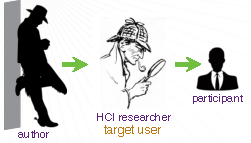
\includegraphics[width=.7\linewidth]{meta-observation}
 	\caption[Meta observation]{Meta observation. An HCI researcher conducts a qualitative study to understand a participant's sensemaking process. This study includes user observation and data analysis. We observe this study to explore its characteristics and identify potential support to HCI researchers -- our target users.}
 	\label{fig:sp-meta-observation}
\end{figure}

In the first meta observation, six participants were recruited and asked to do research online and select the smart watch they would like to purchase. The session stopped when the participant decided on the smart watch model, lasting between 30 to 45 minutes. These sessions were observed by a junior HCI researcher with limited qualitative analysis experience, and he recorded the sensemaking process by making notes on paper and screen recording. Interviews were conducted once the task was completed. Once all six observations were completed, the researcher conducted a \emph{thematic analysis} on the observation data, and the results were summarized in a two-page report. We interviewed the researcher after the report was finished to gain deeper understanding of his qualitative research process.

To ensure the qualitative analysis we observed was not biased, we conducted a second set of meta observations with a more experienced HCI researcher. One participant was tasked to plan a holiday for a fictitious family with particular needs. Two further participants were given the task to select a smart watch as described earlier. This researcher also made notes during the observation, and used thematic analysis to analyze the observation data.

To identify any unique features of qualitative analysis in sensemaking research, we conducted our own thematic analysis on the meta observation data. On completion, we discussed our findings with the two HCI researchers who participated in the meta observations. This led to a qualitative research process that aims to understand sensemaking, consisting of the following steps:

\begin{enumerate}
	\item \textbf{Study Design}. Decide the study setup including the sensemaking task, dataset, and data to capture based on the targeted research question.
	\item \textbf{Data Collection}. Capture the processes while the participants perform their sensemaking tasks. The collected data could include screen captures, think-aloud recordings, video recordings of participants' faces and gestures, and interview notes.
	\item \textbf{Transcription}. Transcribe video and audio recordings verbatim.
	\item \textbf{Coding}. Identify common themes in the transcripts and assign appropriate names or codes to them.
	\item \textbf{Categorization}. Group similar themes into more abstract categories.
	\item \textbf{Model}. Match the identified themes and categories to existing sensemaking models or design a new one, depending on the research question.
\end{enumerate}

Step 2 to 6 represent a progression on the semantics: each step takes the output from the previous step as input, and produces an outcome with richer semantics. This is similar to the four layers of visual analytic activities in the Gotz and Zhou's model (\autoref{sec:lr-analytic-provenance-model}), but targeting a different aspect: the former focuses on the sensemaking model and theory, whereas the latter focuses on user activities. In summary, we did not discover any unique characteristics of qualitative analysis for sensemaking. This implies the approach and tool we developed for sensemaking are likely to be applicable to qualitative analysis intended for other purposes. Our study did equip us with detailed knowledge about the actual qualitative analysis process, which informed the design of our visualization tool.

\subsection{Requirements}
A participatory design session with the two HCI researchers involved in the meta observations was followed up to elicit requirements for the tool that aims to facilitate the existing analysis process. The session discussed possible tool features and designs to address them. The requirements are presented as follows and the design ideas are described in \autoref{sec:sp-design}.
%Our meta thematic analysis led to these requirements:

\begin{enumerate}
	\item \textbf{Thematic analysis support}. This is the analysis method used in both our meta observations and the two sensemaking observations. It also shares many characteristics with other popular qualitative research analysis methods such as grounded theory.

	\item \textbf{Transcription and Coding efficiency}. All aforementioned steps from 2 to 6 are time-consuming; however, \emph{transcription} and \emph{coding} are where a visualization tool can potentially make the most difference. Their lengths largely depend on the efficiency of the tools employed in these steps. \emph{Data collection} primarily depends on the task's completion time and the number of participants. Also, transcription and coding are not as abstract or semantically rich as \emph{categorization} and \emph{model}, making it more feasible to provide automated support.

	%\setcounter{listnum}{\theenumi}
%\end{enumerate}
%
%The participatory design session with HCI researchers led to these requirements:
%
%\begin{enumerate}
%	\setcounter{enumi}{\thelistnum}
	\item \textbf{Existing workflow integration}. The tool should maintain the way researchers currently work and ideally works together with other software packages already used in the analysis workflow.
	\item \textbf{Non-intrusiveness}. The tool should not distract participants or affect their behaviors during the sensemaking tasks.
	\item \textbf{Scalability}. The tool should support reasonably long sensemaking sessions with a duration up to an hour or two.
	\item \textbf{Lightweight}. The tool should be lightweight and support multiple operating systems.

\end{enumerate}
\section{Interface Design}
\label{sec:sp-design}

\subsection{Approach}
The design process started with a close examination of the analysis steps we plan to support. For transcription, we ruled out the possibility of automatic video or audio transcribing because these are research challenges in their own right and require expertise different from visualization and visual analytics. During our meta observation data analysis, we noticed that a large portion of time spent on transcribing video recordings was to identify the sensemaking actions that the participants performed (such as searching) and contextual information associated with these actions (such as the search keyword and its timing). These pieces of information can potentially be captured within the browser, thus considerably reducing transcribing time.

From the aforementioned participatory design session, we found that an important part of the coding process is to understand the sensemaking activities from the video transcripts. For instance, when a participant spent several minutes on a page, he was likely reading through the information. When the participant switched between two pages back and forth, he might be comparing two smart watch models. Understanding the nature of such sensemaking activities; i.e., reading or comparison, is the prerequisite for identifying common themes and naming them. To a certain extent, this is equivalent to inferring ``sub-task'' from ``action'' in the Gotz and Zhou's model. However, this process is difficult to be completely automated~\cite{Dou2009}. After further discussion with the HCI researchers, we identified three important factors to this process that can be supported by visualization:
\begin{enumerate}
	\item \textbf{Seeing the actions before and after the current one}. This provides useful contextual information because an ``action'' is usually a part of a ``sub-task'', which consists of a number of actions. For example, when a participant went through the web page of a number of hotels in succession, they might be comparing these hotels, especially if all these pages are opened from the same hotel booking website. Showing a number of actions together would help a researcher to identify the connections between them and potentially find an interpretation for all the actions in the sequence as a whole.
	\item \textbf{Seeing what a participant was looking at}. It may appear obvious, but it can give a researcher the needed context to understand the sensemaking actions. For example, looking at Google Maps may indicate the participant was trying to locate a certain place. This can be particularly useful if the researcher is absent from the observation.
	\item \textbf{Understanding what a participant was thinking}. Even though this can be partly captured through think-aloud protocol or post hoc interview, another common technique is to enable participants to record their own thinking by providing note taking support.
\end{enumerate}

\subsection{Overview}
SensePath is designed as a Chrome extension consisting of two parts. The first one is a background process running in the participant's browser to automatically capture all the required analytic provenance during the observation stage of the qualitative study. It also offers additional features to add note and highlight text on a web page (Factor 3 -- understanding what a participant was thinking). Besides, participants will not notice any difference from their normal sensemaking session (Requirement 4 -- non-intrusiveness).

The second part is designed to facilitate transcription and coding (Requirement 1 and 2), including a set of four linked visualizations of the captured provenance data (\autoref{fig:sp-overview}) as follows.

\begin{itemize}
\item A \emph{timeline} view displaying participant's sensemaking actions in their temporal order (\autoref{fig:sp-overview}A). This enables researchers to see an action in the context of other actions (Factor 1 -- seeing the actions before and after the current one).
\item A \emph{browser} view showing the web page where the sensemaking action was performed (\autoref{fig:sp-overview}B). This provides the contextual information of sensemaking actions (Factor 2 -- seeing what a participant was looking at).
\item A \emph{replay} view showing screen capture video (\autoref{fig:sp-overview}C). This provides additional contextual information about browser interaction that is missing from the timeline such as scrolling and mouse movement (also Factor 2).
\item A \emph{transcription} view detailing selected sensemaking actions (\autoref{fig:sp-overview}D). The generated transcript can be exported and then used in popular qualitative data analysis software (Requirement 3 -- existing workflow integration).
\end{itemize}

\begin{figure}
 	\centering
 	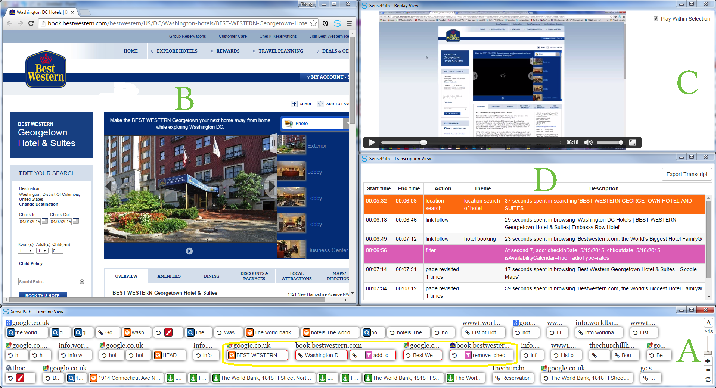
\includegraphics[width=\linewidth]{overview}
 	\caption[Four linked visualizations of SensePath]{Four linked visualizations of SensePath. \textbf{A:} The timeline view shows all captured sensemaking actions in temporal order. \textbf{B:} The browser view displays the web page where an action was performed. \textbf{C:} The replay view shows the screen capture video to provide additional context. \textbf{D:} The transcription view details selected actions (highlighted in the timeline) and generates their transcript.}
 	\label{fig:sp-overview}
\end{figure}

\subsection{Provenance Capture}
\label{sub:sp-provenance}
During the participatory design session, the HCI researchers suggested to capture rich semantic  information that is able to explain the rationale of actions the participant performed. However, this is not always technically feasible. For example, it is possible to detect that a web page has been opened for a long time, but it may be impossible to know whether the participant was reading, thinking, or simply away from the computer screen just by using the information available from the browser alone. Therefore, we agreed to capture the analytic provenance corresponding to the ``action'' level in the Gotz and Zhou's model. This capture can be done automatically yet still provides reasonable amount of semantics to the researchers. We decided to record the following aspects of actions that were regarded useful for qualitative analysis of sensemaking by the HCI researchers, as summarized in \autoref{fig:icon-list}.

\begin{itemize}
	\item \textbf{Type}: When a participant opens a web page, the default type for that action is \emph{browsing}, which lasts until the page becomes inactive. During that period, two common action types are focused: \emph{search \& filter} and \emph{reading}. The former type includes \emph{keyword search}, \emph{location search}, \emph{route search} and \emph{filter}. The latter type includes \emph{highlight} and \emph{annotation}, provided for taking notes and capturing part of the participant's thinking.

	\item \textbf{Timing}: This includes the start and end time of an action.

	\item \textbf{Context}: This contextual information provides additional clues for researchers when looking at individual actions. It varies according to its action type such as the ``keyword'' for search and the ``selected text'' for highlight. Also, the information common for all action types including title, URL, and a screenshot of the rendered web page are always recorded.

	\item \textbf{Relationship}: This provides how a web page was activated with four cases: \emph{revisit} an already opened page, directly \textit{link} from an existing page, manually \textit{type} a new address, and open from a \emph{bookmark}.
\end{itemize}

\begin{figure}
	\centering
	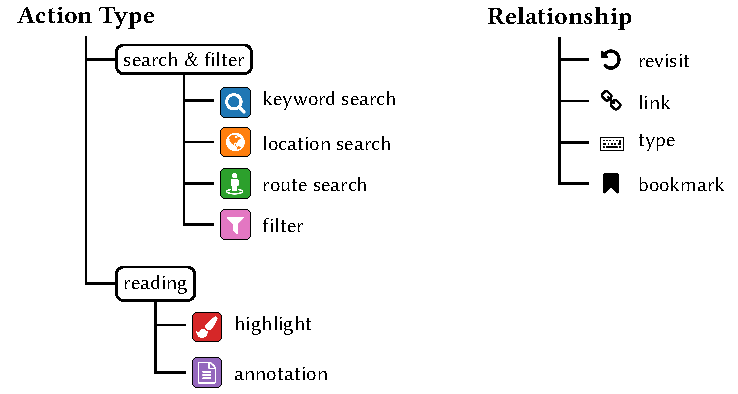
\includegraphics{action-type}
	\caption[Action types and relationships]{All the action types and relationships that SensePath captures, next to the icons representing them.}
	\label{fig:icon-list}
\end{figure}

\subsection{Timeline View}
This view provides an overview of the entire sensemaking process, showing all the captured actions in their temporal order (\autoref{fig:sp-overview}A).

\subsubsection{Visual Representation}
An action is represented as either a bar or a tile, presenting all four aspects of provenance information discussed earlier.

\paragraph{Action Bar}
\autoref{fig:sp-action-bar} shows an example of an \textit{action bar}. The page URL (context) is displayed atop the bar. In the bar, the first icon shows that this action revisited a previously opened page (relationship). Next is the page title (context); only part of which is shown because of the limited space. This is followed by an icon indicating the type of that action such as a ``filter''. \autoref{fig:icon-list} shows all icons representing action types and relationships in SensePath. Note that action type icons have colored background and a black border to distinguish from relationship icons. The last part is the specialized context for each action type, which is filtering parameters in this figure. The width of the action bar corresponds to the length of time spent in browsing the web page, and the relative position of the action type icon marks when the action happened.

\begin{figure}
\centering
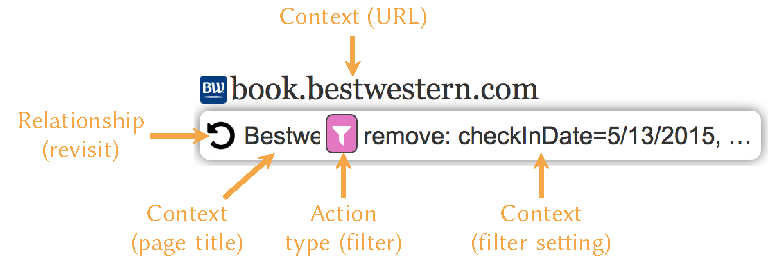
\includegraphics{action-bar}
\caption[An action bar]{An action bar showing all four aspects of provenance information.}
\label{fig:sp-action-bar}
\end{figure}

\paragraph{Action Title}
An \emph{action tile} contains similar analytic provenance information but with more details. \autoref{fig:sp-action-tile} shows the same action as in \autoref{fig:sp-action-bar} but as a tile. Because more height is given, a tile includes a screenshot, which can help the researcher to recognize the web page more effectively. This can also be useful when the researcher was absent from the observation session because she may get a rough context of what the page was about by looking at the its thumbnail. The rest of the provenance information is the same as that in an action bar with more details (e.g., the page title) displayed because of the extra space.

\begin{figure}
\centering
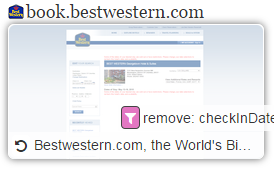
\includegraphics[width=.5\linewidth]{action-tile}
\caption[An action tile]{An action tile complementing the action bar with a page screenshot.}
\label{fig:sp-action-tile}
\end{figure}

The timeline can be shown with either action bars or tiles, interactively controlled by the user. The former is more compact and scalable, whereas the latter shows more details and is suitable for a close inspection. \autoref{fig:sp-timeline-tile} shows an example of timeline with action tiles.

\begin{figure}
\centering
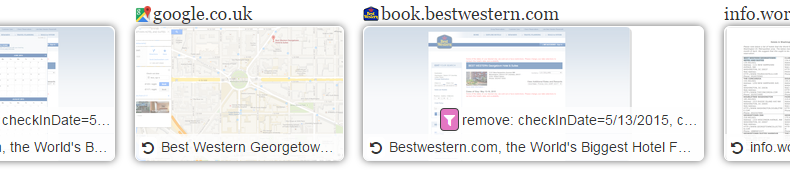
\includegraphics[width=\linewidth]{timeline-tile}
\caption{A part of the timeline with action tiles.}
\label{fig:sp-timeline-tile}
\end{figure}

\subsubsection{Scalability}
\paragraph{Zooming}
Both action bar and tile can reduce their widths through zooming to accommodate more actions. At the smallest level, only the action type is visible, and more details will become available when zooming in. \autoref{fig:sp-timeline-zoom} shows three zoom levels of action bars with the details increasing from top to bottom. The top row shows actions with only icons and a few letters. The middle row reveals the last location search is about ``Best Western'' hotel. The bottom row shows that the first location search is about some ``headquarters'', and the second action is revisiting the ``World bank'' web page. At a low level of detail, only a few letters are shown for each action bar, thus is uninformative. In this case, information richness is sacrificed for scalability. To mitigate this issue, we introduce interactive features such as \emph{selective zooming}, which will be discussed later.

\begin{figure}
\centering
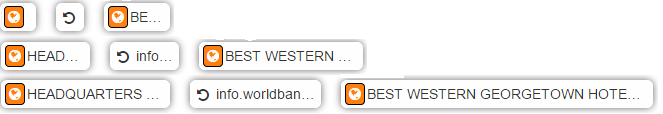
\includegraphics[width=\linewidth]{zoom-3levels}
\caption[Three zoom levels of action bars]{Three zoom levels of action bars with the details increasing from top to bottom.}
\label{fig:sp-timeline-zoom}
\end{figure}

\paragraph{Aggregate Actions}
Instead of showing individual actions, adjacent ones happened on the same web page are merged to save space. It may also help the researcher to quickly understand the participant's process. \autoref{fig:sp-action-bar-merge} shows an aggregated action with eight highlights, which were made on the same Google Plus page.

\begin{figure}
\centering
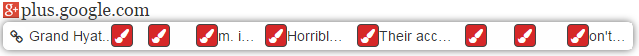
\includegraphics[width=\linewidth]{action-bar-merge-new}
\caption[An aggregate action bar]{An aggregate action bar. It combines eight adjacent highlights made on the same Google Plus page.}
\label{fig:sp-action-bar-merge}
\end{figure}

Because the action bar is short, a timeline can show multiple rows. This, in combination with aggregation and interaction (described next), enables SensePath to display a reasonably large sensemaking session within a limited space. \autoref{fig:sp-overview}A shows about 50 actions out of a total of 70 actions from a 30-minute long session. This addresses Requirement 5 on scalability.

\subsubsection{Interaction}
\paragraph{Mouse Click and Hover}
SensePath includes a number of interactive features to support the analysis of the sensemaking process. Clicking on an action opens the associated web page in the browser view (\autoref{fig:sp-overview}B). This enables researchers to see what the participant was looking at, which is a prerequisite for understanding their thinking. Hovering an action bar highlights other actions happened in the same page with a red border, and brings up a tooltip with additional details such as timing. The example in \autoref{fig:sp-hovering} shows that a page was revisited a number of times during a short sensemaking session.

\begin{figure}
\centering
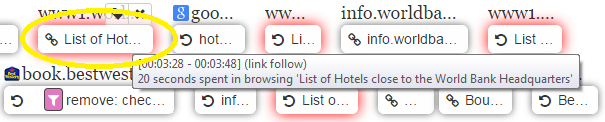
\includegraphics[width=\linewidth]{hovering}
\caption[Mouse hovering effect]{Mouse hovering effect. When an action bar is hovered (highlighted with a yellow eclipse), all other actions with the same URL (red borders) are also highlighted, and a tooltip is showing additional information.}
\label{fig:sp-hovering}
\end{figure}

\paragraph{Selective Zooming}
SensePath implements a focus+context technique~\cite{Cockburn2008} through \emph{selective zooming}: when a zoom is executed, only a selected set of actions affects. This enables researchers to concentrate on certain actions without losing their context. However, they may forget the difference in zoom levels of actions, thus misunderstand the action lengths indicated by the bar widths. SensePath provides a reset button to change the zoom levels of all actions to the default value. \autoref{fig:sp-selective-zooming} illustrates this technique.

\begin{figure}
\centering
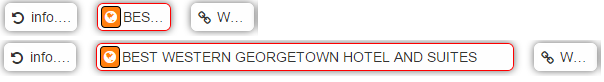
\includegraphics[width=\linewidth]{selective-zooming}
\caption[Selective zooming]{Selective zooming. Selected action bars are with red borders. Top row: before zooming. Bottom row: after zooming -- only the selected action has its zoom level changed.}
\label{fig:sp-selective-zooming}
\end{figure}

\paragraph{Filtering}
Researchers can filter actions based on duration, enabling them to focus on the range of actions they want. For example, if researchers think actions that last only a few seconds are trivial, they can be filtered out using a slider (\autoref{fig:sp-filter}), which sets a minimal length for visible actions. When the slider moves, actions that will be removed fade out, before disappearing when the slider stops. This enables researchers to preview the effect of filtering.

\begin{figure}
\centering
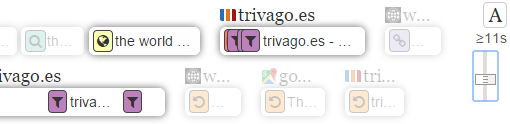
\includegraphics[width=\linewidth]{filter}
\caption[Actions filtering]{Actions filtering. The slider (on the right side) controls the minimal length visible actions. Actions fall below the threshold fade out first before completely disappearing.}
\label{fig:sp-filter}
\end{figure}

\paragraph{Coding}
In traditional qualitative analysis, researchers analyze transcripts to identify common themes and assign suitable names or codes to them. In SensePath, the timeline view provides a succinct summary of the sensemaking process and allows researchers to drill down to explore more specific actions. Representing action types with icons and visualizing a sequence of actions next together may also help researchers to quickly identify patterns of the data, compared to watching videos or reading transcripts. The coding feature is available through a menu button when hovering an action bar. Researchers can assign a code by simply typing it or selecting from a list of previously entered ones.

\subsection{Browser View}
\label{sub:webpage}
When an action is selected in the timeline, its associated web page is shown in the browser view (\autoref{fig:sp-overview}B). This enables researchers to examine the web page that the participant was looking at when performing a sensemaking action. If the action is an annotation or highlight, the browser view will automatically navigate to the location of the web page where the annotation or highlight was made, informing researchers which part of the page the participant was interested in.

\subsection{Replay View}
\label{sub:playback}
SensePath links the timeline to an externally captured screen video to provide additional information about the participant's behavior during the sensemaking session. When a researcher selects an action in the timeline, the replay view automatically jumps to the corresponding part of the screen video when the action is about to start. This avoids manual search within the video, which can be time consuming. After selecting an action in the timeline, a researcher can first check the web page in the browser view and then start the video playback in the replay view if she wants to find out more. The playback automatically stops when it reaches the end of an action, avoiding watching other irrelevant part. Alternatively, the researcher can choose to allow the video to continue; if so, the corresponding action in the timeline will be highlighted as the video progresses.

\subsection{Transcription View}
Detailed information of an action can be revealed by mouse over; however, it is inconvenient to do so for a set of actions. The transcription view addresses this issue by simultaneously presenting the details for all selected actions, in a tabular format (\autoref{fig:sp-overview}D). For each action, this view shows its starting and ending time, action type, assigned themes, and an automatically generated description such as ``37 seconds spent in searching Best Western George Town Hotel and Suites''. This description is based on a predefined template for each different action type with advise from the aforementioned participatory design session. The researchers are allowed to edit the description to better reflect what they think. Row backgrounds match the color of action type icons in the timeline view. The design of this view resembles the transcript interface of popular video transcription software packages to reduce the learning efforts required.

All the information displayed in the transcription view can be exported as a timeline in the SMPTE format~\footnote{ \url{http://en.wikipedia.org/wiki/SMPTE_timecode}}, which can be imported by many popular qualitative data analysis software packages such as InqScribe~\footnote{\url{http://www.inqscribe.com/}} as a transcript. This enables researchers to continue their existing workflows with such software (Requirement 3). Moreover, an SMPTE transcript can be used as a subtitle file in popular video players such as VLC~\footnote{\url{http://www.videolan.org/vlc/index.en_GB.html}}.

\subsection{Implementation}
\label{sub:sp-impl}
This section discuss the architectural design of SensePath and techniques in capturing and detecting provenance.

\subsubsection{Architecture}
SensePath is implemented as a Chrome extension using modern web technologies including HTML5, CSS3, JavaScript and D3.js~\cite{Bostock2011} for visualization. Therefore, it satisfies Requirement 6 about lightweight and support multiple operating systems. Highlight and annotation features require the modification of web page structure, thus they must be implemented as a browser plug-in. We decided to target the Chrome browser first due to its popularity.

SensePath consists of two components: provenance capture and provenance visualization. The capture component relies on content script injected into a loaded web page (to allow highlight and annotation) and the Chrome extension API (to allow automatic action extraction). Therefore, it always works as long as the Chrome extension is enabled. The captured data is exported as a JSON file, which can then be loaded into the visualization component.

The four linked visualizations communicate to each other using the \textit{messaging passing} mechanism provided by the Chrome extension API. When an interaction occurs in one view, it sends a message to notify all other views. Each view constantly listens and responds to such messages. For instance, when an action is selected in the timeline view, it broadcasts that selection. The replay view listens and changes the current time frame of the video to when that action was performed. The replay view uses HTML5 video tag~\footnote{\url{https://developer.mozilla.org/en-US/docs/Web/Guide/HTML/Using_HTML5_audio_and_video}} to display the video capture, thus possible to programmatically set the current playback position to a specific point and to start/pause the playback. The replay view also maintains a list of start/end time of all actions, thus when a video is playing, it finds the action that contains the current time frame and sends a message to the timeline view to highlight it.

\subsubsection{Provenance Capture Techniques}

\paragraph{Search}
Detecting all \emph{search} actions applies URL parsing. When a web page is loaded, its URL is parsed and compared against a set of query templates to check whether a search was performed and to identify its type and parameters. In this prototype, we support automatic detection from many popular web services: keyword search engines (Google, Yahoo, Bing, Ask.com and DuckDuckGo), map search engines (Google Maps, OpenStreetMap and Yahoo Maps), social networking websites (Facebook and Twitter), e-commerce websites (Amazon and ebay) and hotel booking websites (Booking.com and Expedia). All these web services follow their own query templates and expose all necessary parameters in the URLs, allowing extracting the required information from them. The following examples show the query templates and parameters:

\begin{itemize}
	\item Google keyword search: \texttt{https://www.google.com/search?\textbf{q=\{keyword\}}}
	\item Yahoo Maps route search: \texttt{https://maps.yahoo.com/directions/?\\\textbf{o=\{source\}\&d=\{destination\}}}
\end{itemize}

SensePath uses a structure with three parameters to represent these templates, including a host name (\texttt{www.google.}), a path name (\texttt{/search}) and a regular expression (\verb|/\Wq=([\w%+]*)/i|) for keyword extraction. Adding detection support to other services only requires the knowledge of these three parameters.

\paragraph{Filter}
Detecting \emph{filter} actions also uses URL parsing as in detecting \emph{search} actions but does not require prior knowledge about query templates. We apply a heuristic that if two consecutive URL requests share the same host name and path name but different parameters, the second page is the result of a filtering action on the first one. More specifically, a URL is compared against its previous URL within the same tab; if they have the same host name and path name, their query strings are parsed to a collection of key/value pairs. For each key, three cases can happen when comparing its value between the previous and the current URL:

\begin{itemize}
	\item \textbf{add}: The key was absent from the previous URL but is added to the current one.
	\item \textbf{remove}: The key was present in the previous URL but is removed from the current one.
	\item \textbf{update}: The key is present in both URLs but their values are different. Note that if their values remain unchanged, it is unnecessary to report.
\end{itemize}

For example, considering these two consecutive URLs:
\begin{enumerate}
	\item \url{hotel.com/search?loc=london&guests=1}
	\item \url{hotel.com/search?loc=london&guests=2&checkIn=2015%2F10%2F24}
\end{enumerate}

Following our heuristic of comparing URLs, this filter action can be captured as ``\texttt{add:} \texttt{\{checkIn=2015/10/24\}, update:} \texttt{\{guests=1$\rightarrow$2\}}'', and may be interpreted as ``the participant set a new check-in date and changed the number of guests from 1 to 2''.

\paragraph{Limitations} Both \emph{highlight} and \emph{annotation} actions are implemented using the content script~\footnote{\url{https://developer.chrome.com/extensions/content_scripts}} in the Chrome extension API, thus all information needed can be saved. To allow revisiting to the exact location where a passage of text is highlighted, the relative location of its DOM element to the root element of the web page is captured. However, when the web page structure is changed, the recorded position might become invalid, leading to inaccurate recovery.

All the heuristics applied for search and filter actions only work if web services expose their parameters in the URL. In other words, our method fails to work if POST or AJAX requests are used. So far, for all services we planned to support, we have never encountered such a case. For example, Google Maps uses AJAX calls to load map tiles, but all the information we want to extract is available in the URL. Also, most popular online services use GET instead of POST requests. It is actually possible to support web services that encode the required information in POST or AJAX requests by monitoring all the communication between the browser and the server, not just the changes in URL. However, this requires considerably more implementation effort and is only possible with open source browsers such as Firefox and Chrome that provide access to all client-server communication.

For GET requests, it is also infeasible to extract the meaning of URL parameters if they are encoded. We encountered one such case, Bing Maps, which encodes query parameters as HEX strings. For example, this lengthy URL, \url{https://www.bing.com/maps/#Y3A9NTEuNTkwMTk5fi0wLjIyNTAw...}, is the URL produced by searching for ``london''.

To guarantee an exact restoration of a visited web page, it is necessary to save a static copy of the web page when an action happened. This is similar to the \emph{P-Set model}~\cite{Jankun-Kelly2007} for visualization exploration where the visual transforms, parameters, and results are stored for fully describing and reproducing the performed process. However, for simplicity, we only capture the action type (i.e., visual transforms) and context (i.e., parameters), but not the resulting web page (i.e., results). The browser snapshot and computer screen video are captured to compensate for this limitation to a certain extent.

\subsubsection{Trade-off in Provenance Capture}
The SensePath extension only captures user actions performed on the web browser, excluding all other types of provenance data to satisfy Requirement 6 -- lightweight. Screen capture can be done separately using another software such as QuickTime~\footnote{\url{https://support.apple.com/quicktime}}. Similarly, if the researchers have an interest in understanding which part of the screen a participant was looking at, eye tracking can be performed with an additional software. There might be no limit in capturing provenance information (such as face/gesture/brain tracking) for a comprehensive study of the sensemaking process performed by a participant. However, adding too many extra devices to capture provenance might affect the way participants perform their tasks. Therefore, we decided to take a lightweight approach to increase the application of SensePath.
\section{Evaluation}

We conducted two user-centered evaluations: the first one is to investigate how SensePath is used by a domain expert, and the second one is to discover whether SensePath has any potential advantages compared with a traditional method. We first conducted a number of user studies of participants carrying out an online sensemaking task to establish a ground truth dataset. Then, we recruited HCI researchers to analyze the sensemaking processes of these participants. In this section, we regard these HCI researchers as ``analysts'' and people performing sensemaking tasks as ``participants'' or ``sensemakers''.

We recruited two participants to take part in this study: a post-doctoral researcher and a PhD student, both males. Participants were given the same task, which was to use the Chrome browser to find appropriate accommodation for two academics attending a conference at the World Bank headquarters in Washington, D.C. We provided participants with information about the location and dates of the conference, but gave no further details in the scenario to maintain suitable complexity in the task, and to ensure it was as realistic as possible.

Both participants were given 30 minutes to perform the task. Throughout the study, their sensemaking actions were collected within SensePath, and their screens were also recorded using a commercial software. We also encouraged participants to think aloud throughout the study, and finally conducted a semi-structured interview asking them to reveal:

\begin{itemize}
	\item The rationale behind their choice
	\item The strategy in approaching the task
	\item The process they went through in executing that strategy
\end{itemize}

\subsection{Evaluation 1}

\subsubsection{Design}
The goal of this evaluation is to explore how SensePath is used by a domain expert performing a real-world task. We recruited an analyst with seven years of experience in qualitative research to analyze the actions captured in the sensemaking process outlined earlier using SensePath. We gave the analyst a short tutorial to introduce and explain features of SensePath, before practicing with a trial task. She was provided with a laptop running SensePath, connected to an external monitor, providing a multi-screen setup as in \autoref{fig:sp-evaluation-setup}. During the analysis, we encouraged the analyst to provide feedback through a think-aloud protocol. We recorded her responses and other observations using written notes. At the end of the analysis, we asked the analyst to complete a discovery sheet reporting her findings. A semi-structured interview was followed up to gain deeper understanding of her experience. The discovery sheet included the following questions:
\begin{itemize}
	\item Identify the sensemaker's strategy in approaching the task and characteristics demonstrating that.
	\item Identify the steps the sensemaker took in choosing suitable accommodation and provide a name (code/theme) for each step.
	\item Identify any interesting patterns in the data.
\end{itemize}

\begin{figure}[!htb]
\centering
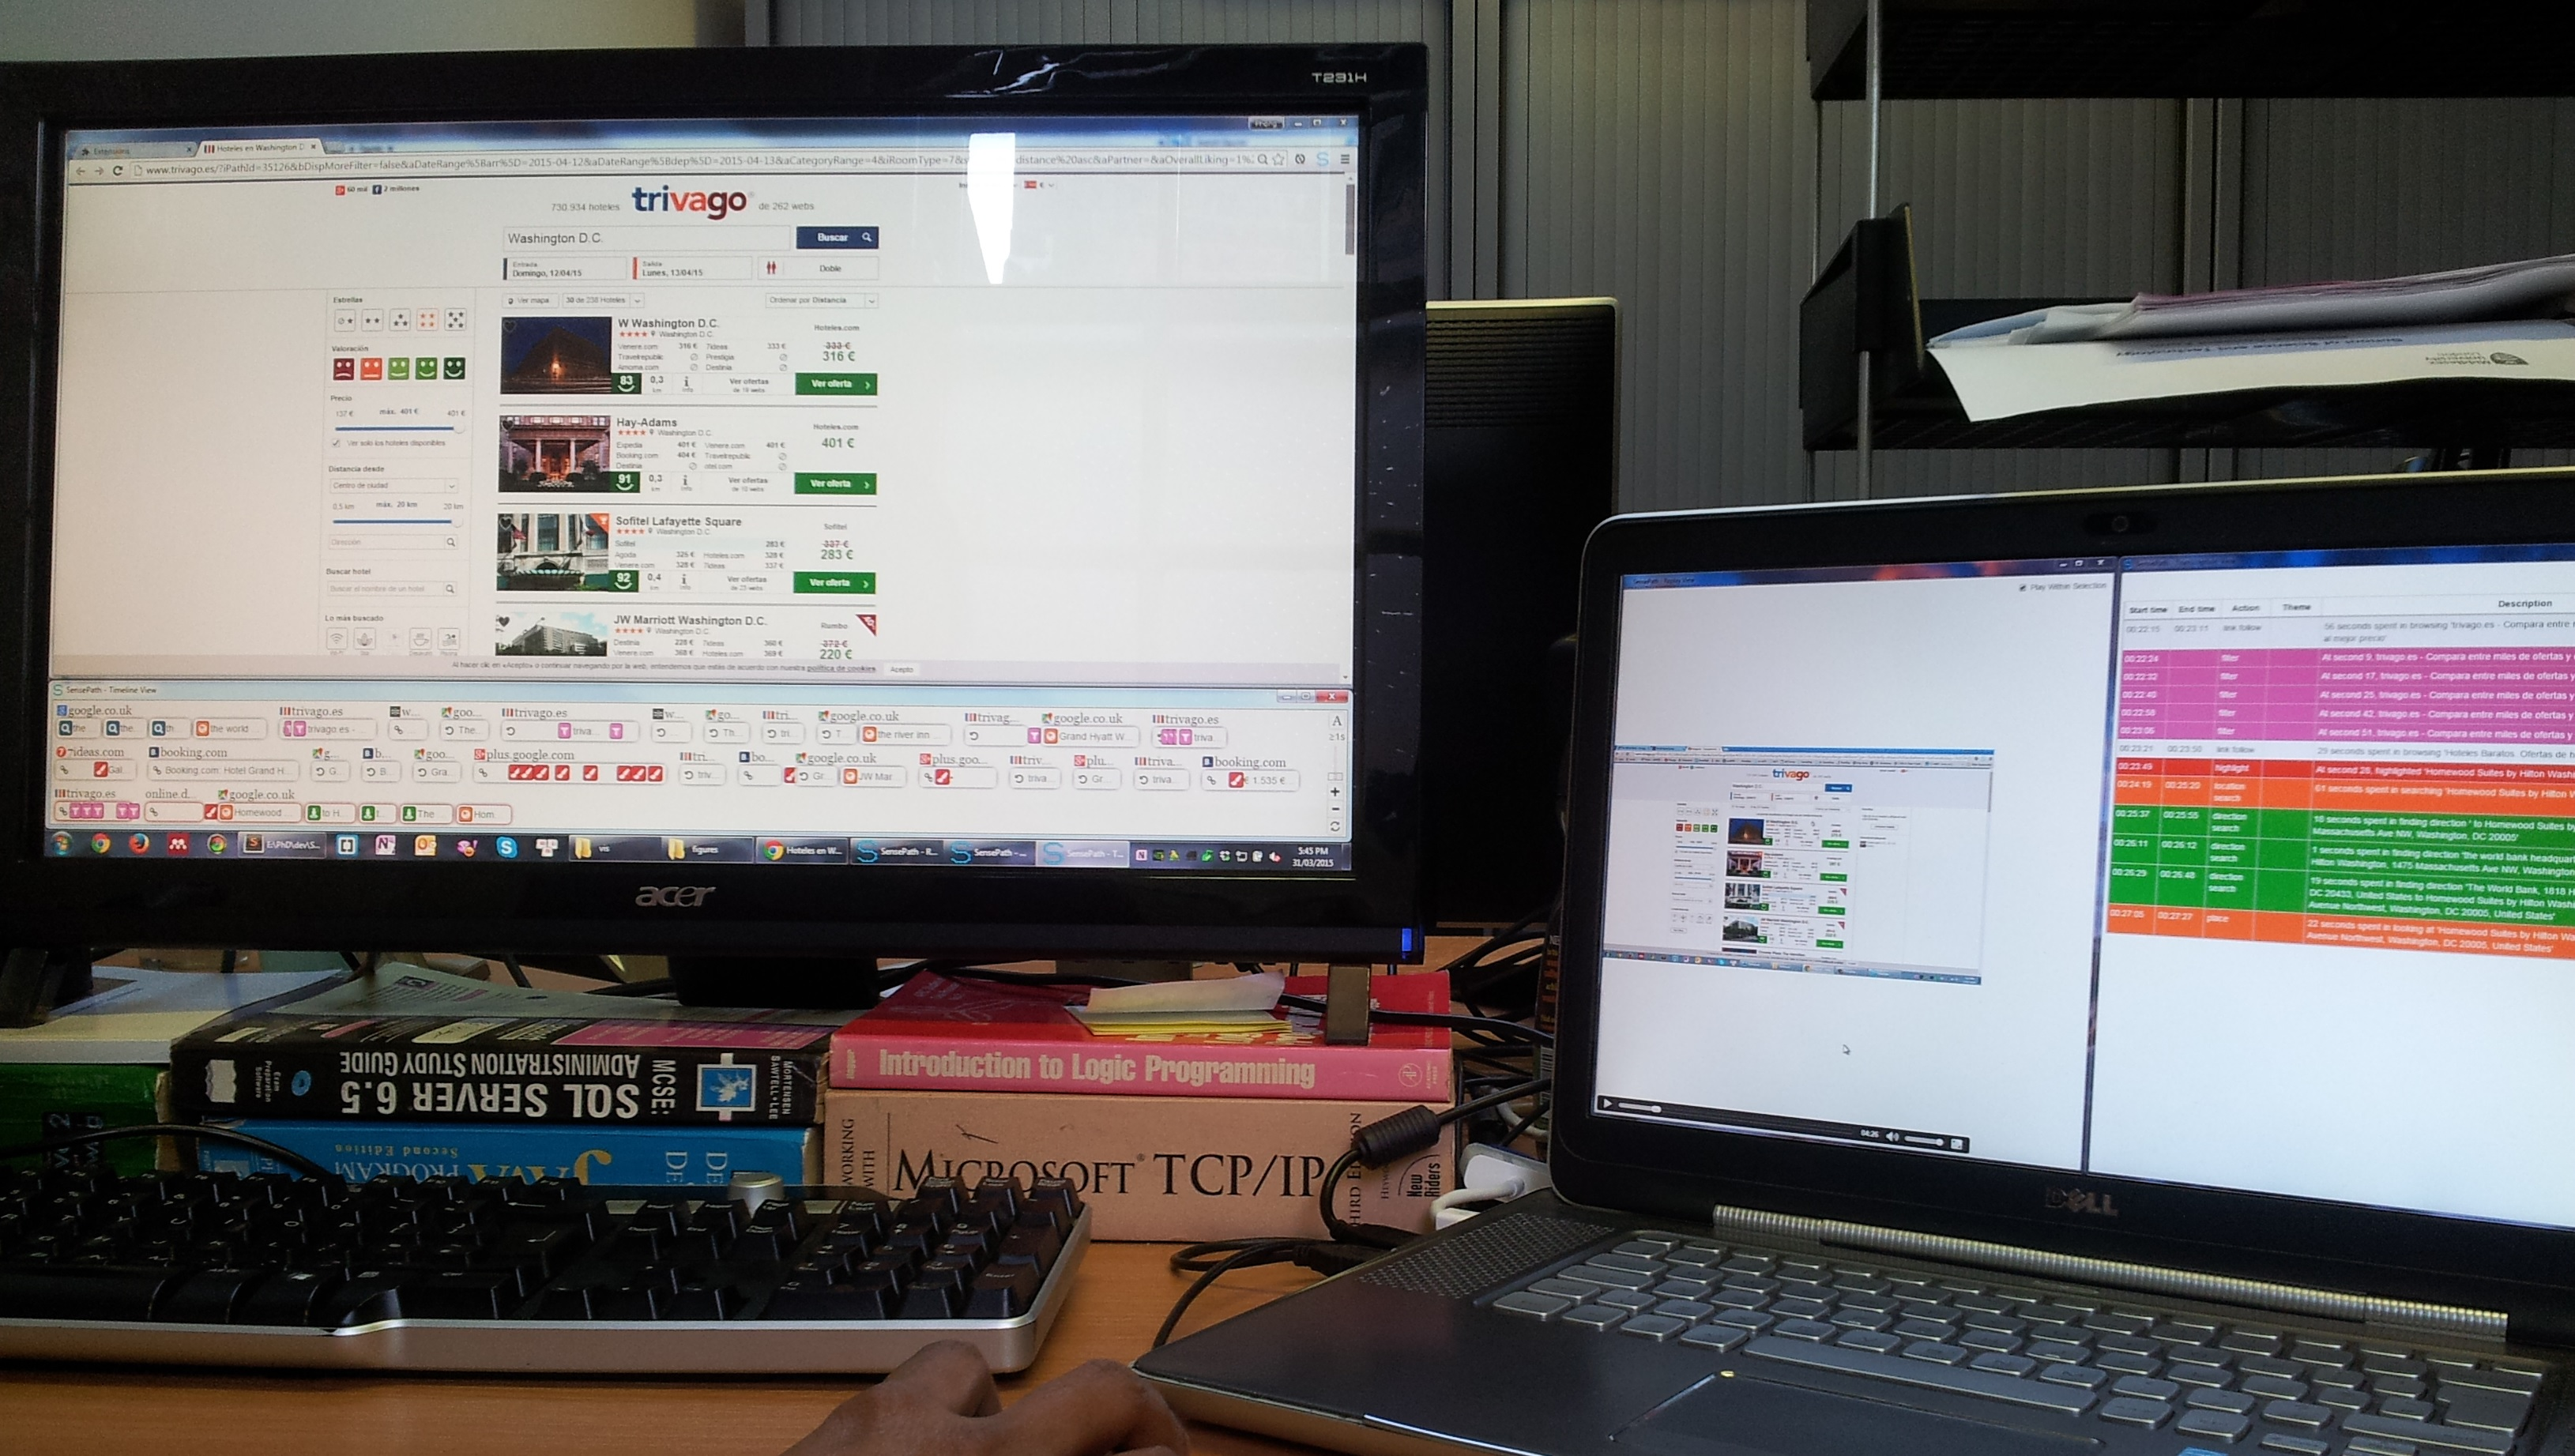
\includegraphics[width=\linewidth]{experiment-setup}
\caption[The setup of the qualitative analysis with SensePath]{The setup of the qualitative analysis with SensePath. The monitor on the left shows the timeline and browser views, and the laptop on the right shows the replay and transcription views.}
\label{fig:sp-evaluation-setup}
\end{figure}

\subsubsection{Findings}
The analyst took approximately one hour to analyze 30 minutes of study data. This shows a reduction of half the time taken using SensePath compared with traditional methods of video analysis, which would typically take around four hours of analysis for every hour of study data~\cite{Burr2006}.

The analyst initially used the timeline to view sensemaking actions at a low resolution, before focusing on interesting parts of the data in more detail. Because these actions are visualized in a single view, the analyst reported she could quickly make an initial summary assessment of the sensemaker's overall performance of the task, before identifying potentially interesting behaviors in the data. One such example of this is when she saw many highlights on a Google Plus page, next to each other in the timeline, she said ``It seems that the guy [the sensemaker] found interesting information on that [Google Plus] page because he highlighted a lot there''. She then moved the mouse over these highlight icons to read the highlighted text shown in the tooltips. Interestingly, she quickly concluded that ``He only focused on negative reviews''. She clicked on some of those icons to open up the Google Plus page to gain more context. Unfortunately, that page is content-dynamic, thus some highlighted texts failed to be reselected. She switched to watch the video in the replay view and heard that the participant was talking to us about his preference to negative reviews (we used think-aloud protocol), which confirmed her initial judgment. She also mentioned that offering highlight feature to the sensemakers is useful because it enables her to quickly identify their interests.

To understand the whole sensemaking process, the analyst quickly went through all the actions shown in the timeline. The analyst was able to successfully describe the steps taken by the sensemakers in approaching to the task. We confirmed those steps were all correct by re-watching the capture video and verifying with the sensemakers. \autoref{fig:sp-evaluation-diagram} shows a reproduction of a written diagram created by the analyst illustrating the steps she identified. She explained the diagram to us; for instance, ``that guy searched for the address of the headquarters, then viewed it in Google Maps to get a sense of where it is''.

\begin{figure}[ht]
\centering
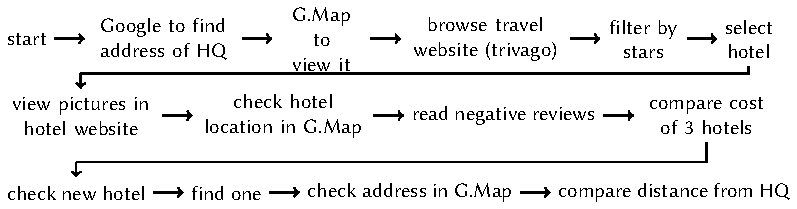
\includegraphics{diagram}
\caption[Sensemaking steps]{Sensemaking steps. A reproduction of diagram written by the analyst during the evaluation illustrating the steps taken by the sensemaker in the task.}
\label{fig:sp-evaluation-diagram}
\end{figure}

The analyst reported that using the timeline view she could easily identify interesting recurring patterns because all actions are shown together. As an example for such patterns, when the sensemaker found a hotel in a booking website, he looked at its pictures first, then searched for its location in Google Maps, and checked its route to the headquarters. The sensemaker repeated this process for several hotels he found.

The analyst managed to find an overall strategy that the sensemaker applied in approaching the task: he targeted reasonably cheap hotels (evidenced by filtering out 5-star ones) and considered hotels close to the headquarters (supported by putting them in Google Maps for comparison). This confirmed with what the sensemaker told us: as a professional academic, he wanted to save money for the university, but also did not want to stay too far away from the conference venue.

The analyst commented that the video and audio recordings were intrinsic to carry out a fuller, more detailed analysis by providing additional information that was unavailable in the timeline and the browser views such as mouse movement or page scroll interactions. Therefore, the replay view helped her gain further insight into the sensemaker's behaviors. Because the analyst did not have to watch the whole video, she thought that she could save valuable time in the analysis. Moreover, she stated that as clicking on an action in the timeline view skipped to the relevant place in the screen capture, further time was saved in scrubbing through the video, which often happened in her experience of analyzing video data. For example, when seeing a long search action bar, she knew that the sensemaker spent much time in Google Maps, searching for a specific location; however, what exactly he was doing is neither available in the timeline nor the browser view. Thus, she needed to watch the video to get more information.

\subsection{Evaluation 2}

\subsubsection{Design}
The goal of this evaluation is to establish an initial understanding of whether SensePath has any advantages compared with a traditional method. We conducted an experiment with two senior HCI researchers to analyze a short 15-minute video (part of the video used in the first evaluation) using thematic analysis, but only for the first two stages: transcription and coding, which SensePath is designed to support. One analyst used SensePath and the other used a transcription software called \textit{Transcription} ~\footnote{\url{https://code.google.com/p/transcriptions/}}. This tool shows the transcribing video and a text editor side by side, and provides a set of shortcuts for quick video manipulation such as pause/play or step forward/backward. This enables users to control the video play while focusing on the editor to type in the transcript, thus accelerates the transcription. The experiment setup and procedure were the same as in the first evaluation. The analysts were asked to produce a transcript of the video, identify the steps the sensemaker took in performing the task, and assign codes for them. Timing for each analysis stage was recorded, and an interview was followed after the analysis to gain deeper understanding of their processes.

\subsubsection{Findings}
The result showed that SensePath can significantly reduce time for transcription. In the baseline condition, it took the analyst 60 minutes to transcribe the video, about 15 minutes of them spent for the think-aloud audio. In SensePath condition, transcribing was done automatically, and it took the analyst 5 minutes to traverse all actions in the timeline to get a sense of the sensemaker's process.

In regard to accuracy, SensePath identified 39 actions and all are correct (each action is verified by us). In the baseline condition, the analyst identified additional actions that SensePath was unable to capture because the browser did not reload such as ``click on a pull-down menu to see more options'' or ``encircle the rating point with mouse movement''. However, he missed two actions that were correctly identified by SensePath: ``set checkin and checkout date'' and ``change sorting criteria''.

Watching the video helped the analyst transcribe with richer information. For instance, SensePath can only record where a web page came from such as manually typing the address or linking from another page. Whereas in the baseline condition, more context can be added such as which button was clicked to open that new page. However, SensePath can save time from transcribing long text such as for highlights or annotations.

For coding, in the baseline condition, the analyst copied the transcript to Excel and assigned codes in a column next to the text. The analyst using SensePath can directly assigned codes to actions in the timeline view. SensePath was only slightly faster than the traditional method (40 minutes vs. 45 minutes). It could because the analyst using SensePath needed to familiarize himself with the data by watching some parts of the video a few times, whereas the other analyst already spent long time watching the video during the transcription stage.

In both conditions, the analysts produced reasonable and comparable codes for the steps they identified. For example, in the baseline condition, the analyst created codes such as ``Google search for location'', ``drill down'', ``assessment'' and ``assessing relevance of evidence''. The analyst with SensePath produced similar codes including ``looking for headquarters location'', ``locate option'', ``assess proximity'', ``assess price'' and ``assess reviews''.

Similar to the analyst in the first evaluation, the analyst with SensePath also quickly went through all sensemaking actions to have an overview of the process, before drilling down to actions of interest. Especially, the analyst often used actions in the timeline as a navigation to the part of the video he wanted to watch. He said he needed to watch some parts of the video several times to understand the intention of the sensemaker, and clicking on the actions enables him to quickly go to the correct part.
\section{Summary}
This chapter introduces a visualization tool SensePath enabling users, specifically HCI researchers, to explore reasoning relationships of the sensemaking processes performed by other people. It facilitates thematic analysis of semi-automatic provenance data for online sensemaking tasks, targeting the transcription and coding phases. The data is visualized in four linked views: timeline, browser, replay and transcription. The timeline provides an overview of the sensemaking process and can support a reasonably long sensemaking session common in qualitative research observations. The browser view shows the web page the participant was looking at when performing a sensemaking action, and is complemented by the replay view with the screen capture video of the action. The transcription view provides all the details for a set of actions and can export the information in a format compatible with popular qualitative analysis software packages, so that analysts can continue working in their existing workflow.

An evaluation was conducted with an experienced qualitative researcher, who found many features of SensePath helpful for her work, and the data collected from the observation showed that SensePath met most of the requirements it set out to achieve. Another evaluation with two HCI researchers suggested the potential of improvement in completion time for SensePath in the transcription and coding phases.

SensePath can be extended to support exploring reasoning relationships in other domains beyond online sensemaking tasks. The visualization component can be reused straightforwardly. However, the capture component of SensePath is currently tightly associated with extracting sensemaking actions in a web page, thus needs to be updated. Of course, a discussion with targeted users is required to understand what actions and information are important to capture.  Also, to make SensePath more accessible for non-technical users (such as the analysts) in adding automatic detection of ``search'' actions from new web services, a simple graphical interface can be built to allow such an update.

Considering the qualitative user study as a specific sensemaking task, SensePath visualizes analytic provenance allowing researchers to gain understanding into the sensemaking processes performed by other people. The next chapter will investigate how to support the sensemaking users themselves in solving their problems through visualization of their analytic provenance data.